\chapter{NMR in de diepte: pulsen, relaxatie en 2D}\label{ch:b3:advanced-nmr}

Een MRI-scanner in een ziekenhuis en de NMR-spectrometer van een
scheikundefaculteit werken volgens hetzelfde principe. Beide plaatsen
waterstofkernen in een sterk magneetveld, kantelen hun magnetisatie met
een korte puls radiogolven, en luisteren naar het zwakke signaal dat ze
induceert terwijl ze precedeert en relaxeert. De scanner maakt van het
signaal een beeld van zacht weefsel; de spectrometer een lijst van
chemische verschuivingen en koppelingen, en, met meerdere pulsen na
elkaar, tweedimensionale kaarten die laten zien welk atoom aan welk
gebonden is. Dit hoofdstuk legt uit wat de pulsen doen, waarom het
signaal uitdooft, en hoe tweedimensionale spectra gelezen worden --- de
methode waarmee de meeste nieuwe organische structuren tegenwoordig
opgehelderd worden.

\begin{recall}
Het deel van jaar~1 interpreteerde ${}^1$H-NMR-spectra: chemische
verschuiving, afscherming, equivalente protonen, integratie,
spin-spinkoppeling, koppelingsconstanten en multipletten. Het deel van
jaar~2 voegde ${}^{13}$C-NMR toe met breedbandontkoppeling en DEPT, waarvan
het de pulssequentie als gegeven aannam; de pulsen worden hier
uitgelegd.
\Cref{ch:b3:many-electron-atoms} behandelde spin als een impulsmoment. Uit
de natuurkunde: een magnetisch moment in een veld heeft de energie $-\boldsymbol\mu\cdot\mathbf B$, en
bezettingen van niveaus volgen de boltzmannfactor $\eu^{-\Delta E/kT}$, uitgewerkt
in \cref{ch:b3:partition-functions}.
\end{recall}

\begin{omfigure}
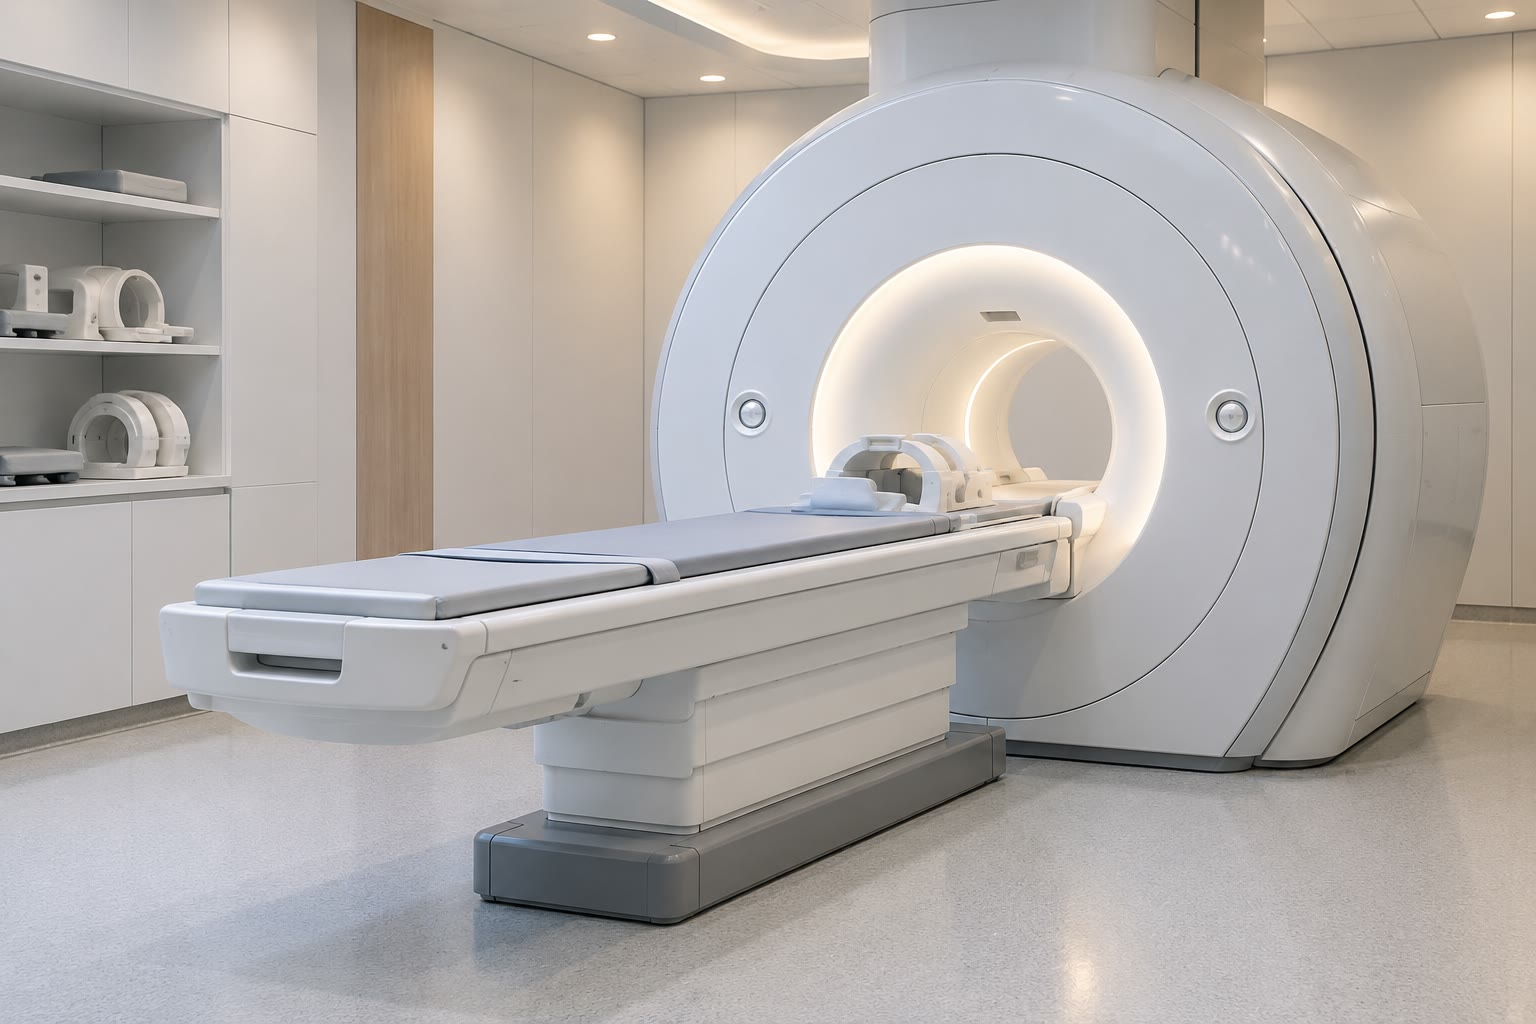
\includegraphics[width=0.52\linewidth]{images/book4/ai/b3-08-mri.jpg}\hspace{0.8em}%
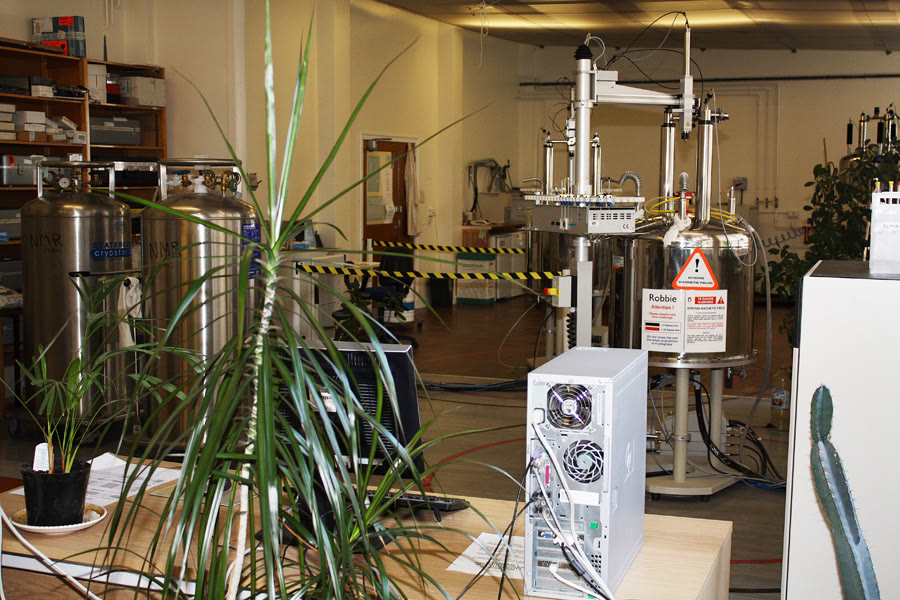
\includegraphics[width=0.4\linewidth]{images/book4/nmr-lab.jpg}

{\small Links: een MRI-scanner in een ziekenhuis. Rechts: een
NMR-laboratorium; elke supergeleidende magneet staat in zijn cryostaat, die
bijgevuld wordt met vloeibaar helium en vloeibare stikstof uit de
dewarvaten links. Foto Shandchem, CC BY 2.0.}
\end{omfigure}

\section{Kernspins in een magneetveld}

\begin{definition}[Kernspinkwantumgetal, gyromagnetische verhouding]\label{def:b3:advanced-nmr:nuclear-spin}
Een kern heeft een spinimpulsmoment met kwantumgetal $I$, zijn
\emph{kernspinkwantumgetal}\index{kernspinkwantumgetal} ($I = 0$
voor \ce{^{12}C}, \ce{^{16}O}; $\frac12$ voor \ce{^1H}, \ce{^{13}C}, \ce{^{15}N}, \ce{^{19}F},
\ce{^{31}P}; 1 voor \ce{^2H}, \ce{^{14}N}), en een magnetisch moment $\boldsymbol\mu = \gamma\hat{\mathbf
I}$ dat ermee evenredig is; $\gamma$ is de
\emph{gyromagnetische verhouding}\index{gyromagnetische verhouding}.
Langs een veld $B_0$ (as $z$) neemt $\hat I_z$ de waarden $m_I\hbar$ aan,
$m_I = -I, \dots, I$.
\end{definition}

\begin{proposition}[Zeemanniveaus]\label{prop:b3:advanced-nmr:zeeman}
In een veld $B_0$ zijn de niveaus $E_m = -m_I\gamma\hbar B_0$; de overgangen $\Delta m_I = \pm1$
absorberen bij de frequentie
\[
\nu_0 = \frac{\gamma B_0}{2\pi}.
\]
\end{proposition}

\begin{proof}
$E = -\boldsymbol\mu\cdot\mathbf B = -\gamma B_0\hat I_z$, met \omterm{def:b3:quantum-model-systems:operator}{eigenwaarden} $-\gamma B_0m_I\hbar$. Naburige
niveaus verschillen met $\gamma\hbar B_0 = h\nu_0$.
\end{proof}

\begin{definition}[Larmorfrequentie]\label{def:b3:advanced-nmr:larmor}
$\nu_0 = \gamma B_0/2\pi$ is de \emph{larmorfrequentie}\index{larmorfrequentie} van de
kern: de resonantiefrequentie, en ook de frequentie waarmee zijn
magnetisch moment om het veld precedeert.
\end{definition}

\begin{example}[De gangbare kernen]\label{ex:b3:advanced-nmr:nuclei}
% ledger: const:gammaP, nuc:C13.mu, nuc:F19.mu, nuc:P31.mu, nuc:N15.mu, const:muN
Voor een kern met spin $\frac12$ en moment $\mu$ is $\gamma/2\pi = \mu/(Ih) = 2\mu/h$. Met de
gemeten momenten: \ce{^1H} \qty{42.58}{MHz/T}, \ce{^{19}F} \qty{40.08}{MHz/T}, \ce{^{31}P}
\qty{17.25}{MHz/T}, \ce{^{13}C} \qty{10.71}{MHz/T}, \ce{^{15}N} \qty{-4.32}{MHz/T}. Een
``spectrometer van \qty{400}{MHz}'' heeft $B_0 = \qty{9.4}{T}$: zijn protonen
resoneren bij
\qty{400.2}{MHz}, zijn koolstofkernen bij \qty{100.7}{MHz}.
\end{example}

\begin{proposition}[Een minuscuul bezettingsverschil]\label{prop:b3:advanced-nmr:populations}
Voor spin $\frac12$ bij temperatuur $T$ is het overschot aan kernen in het
lagere niveau
\[
\frac{N_\alpha - N_\beta}{N} \approx \frac{\gamma\hbar B_0}{2kT}.
\]
\end{proposition}

\begin{proof}
$N_\beta/N_\alpha = \eu^{-\Delta E/kT} \approx 1 - \Delta E/kT$, omdat $\Delta E \ll kT$; dus
$(N_\alpha - N_\beta)/(N_\alpha + N_\beta) \approx \Delta E/2kT$, met $\Delta E = \gamma\hbar B_0$.
\end{proof}

Voor protonen bij \qty{9.4}{T} en \qty{300}{K} is het overschot \num{3.2e-5}:
slechts drie kernen op honderdduizend dragen bij. Omdat zowel het overschot
als de in de spoel geïnduceerde spanning groeien met $\gamma$ en $B_0$,
groeit het signaal ruwweg als $\gamma^3B_0^2$: de reden voor steeds sterkere
magneten, en voor de lage gevoeligheid van kernen met een kleine $\gamma$
en een lage natuurlijke abundantie, zoals
\ce{^{13}C}.

\section{Pulsen en het vrije-inductieverval}

\begin{definition}[Netto magnetisatie, roterend assenstelsel]\label{def:b3:advanced-nmr:magnetisation}
De \emph{netto magnetisatie}\index{netto magnetisatie} $\mathbf M$ van een
monster is de som van zijn kernmagnetische momenten per volume-eenheid; in
evenwicht is ze
$M_0$ langs $\mathbf B_0$. Het \emph{roterend assenstelsel}\index{roterend assenstelsel}
is een stel assen $x'$, $y'$, $z$ dat om $z$ draait met de frequentie van
de aangelegde radiogolven; daarin ziet men de precessie bij $\nu_0$
vertraagd tot de offset $\nu_0 -
\nu_{\mathrm{rf}}$.
\end{definition}

\begin{proposition}[Precessie]\label{prop:b3:advanced-nmr:precession}
Een magnetisatie in een veld gehoorzaamt aan $\dd\mathbf M/\dd t = \gamma\,\mathbf M\times\mathbf B$; in een
statisch veld $B_0\mathbf e_z$ draait haar transversale component om $z$
met de hoekfrequentie $\omega_0 = \gamma B_0$, terwijl $M_z$ constant blijft.
\end{proposition}

\begin{proof}[Gedeeltelijk bewijs]
De vergelijking is de klassieke krachtmomentvergelijking voor een
magnetisch moment met een impulsmoment, hier uit de natuurkunde
overgenomen. Met $\mathbf B = B_0\mathbf e_z$: $\dot M_x = \gamma
B_0M_y$, $\dot M_y = -\gamma B_0M_x$, $\dot M_z = 0$, met als oplossing $M_x + \iu M_y \propto
\eu^{-\iu\gamma B_0t}$: een rotatie met $\omega_0$ (met de klok mee gezien
vanaf $+z$ voor $\gamma > 0$).
\end{proof}

\begin{definition}[Radiofrequente puls, kantelhoek]\label{def:b3:advanced-nmr:pulse}
Een \emph{radiofrequente puls}\index{radiofrequente puls} is een korte stoot
radiogolven bij $\nu_{\mathrm{rf}} \approx \nu_0$, waarvan het magneetveld
$B_1$, vast in het \omterm{def:b3:advanced-nmr:magnetisation}{roterende assenstelsel} langs $x'$, $\mathbf M$ om $x'$
doet draaien. De gedraaide hoek is de
\emph{kantelhoek}\index{kantelhoek} $\theta = \gamma B_1t_p$ voor een puls
met duur
$t_p$: een puls van $90^\circ$ brengt $\mathbf M$ in het $x'y'$-vlak, een
puls van $180^\circ$ keert
haar om.
\end{definition}

\begin{omfigure}
\tdplotsetmaincoords{70}{120}
\begin{tikzpicture}[tdplot_main_coords, font=\small, >=Stealth]
  \begin{scope}
    \draw[->, gray] (0,0,0) -- (1.8,0,0) node[anchor=north east] {$x'$};
    \draw[->, gray] (0,0,0) -- (0,1.8,0) node[anchor=north west] {$y'$};
    \draw[->, gray] (0,0,0) -- (0,0,1.8) node[anchor=south] {$z$, $\mathbf B_0$};
    \draw[->, omThm, very thick] (0,0,0) -- (0,0,1.4) node[anchor=west] {$\mathbf M$};
    \node[anchor=north] at (0,0,-0.9) {evenwicht};
  \end{scope}
  \begin{scope}[shift={(0,4.6,0)}]
    \draw[->, gray] (0,0,0) -- (1.8,0,0) node[anchor=north east] {$x'$};
    \draw[->, gray] (0,0,0) -- (0,1.8,0) node[anchor=north west] {$y'$};
    \draw[->, gray] (0,0,0) -- (0,0,1.8) node[anchor=south] {$z$};
    \draw[->, omDef, thick] (0,0,0) -- (1.2,0,0) node[anchor=south east, xshift=-2pt] {$\mathbf B_1$};
    \draw[->, omThm, very thick] (0,0,0) -- (0,1.4,0) node[anchor=south west] {$\mathbf M$};
    \node[anchor=north] at (0,0,-0.9) {na een puls $90^\circ_{x'}$};
  \end{scope}
  \begin{scope}[shift={(0,9.2,0)}]
    \draw[->, gray] (0,0,0) -- (1.8,0,0) node[anchor=north east] {$x'$};
    \draw[->, gray] (0,0,0) -- (0,1.8,0) node[anchor=north west] {$y'$};
    \draw[->, gray] (0,0,0) -- (0,0,1.8) node[anchor=south] {$z$};
    \draw[->, omThm, very thick] (0,0,0) -- (0,0,-1.4) node[anchor=west] {$\mathbf M$};
    \node[anchor=north] at (0,0,-1.6) {na een puls $180^\circ_{x'}$};
  \end{scope}
\end{tikzpicture}

{\small De magnetisatie in het \omterm{def:b3:advanced-nmr:magnetisation}{roterende assenstelsel}. Een puls van
$90^\circ$ om $x'$
draait $\mathbf M$ van $z$ naar $y'$ (met $\gamma > 0$ volgt de rotatie de
linkerhandregel om $\mathbf B_1$, de gebruikelijke conventie); een puls van
$180^\circ$ keert haar om.}
\end{omfigure}

\begin{definition}[Vrije-inductieverval]\label{def:b3:advanced-nmr:fid}
Na een puls van $90^\circ$ precedeert de transversale magnetisatie met de
\omterm{def:b3:advanced-nmr:larmor}{larmorfrequentie} en induceert ze een oscillerende spanning in de spoel
rond het monster, die uitsterft naarmate de magnetisatie relaxeert: het
\emph{vrije-inductieverval}\index{vrije-inductieverval} (FID).
\end{definition}

\begin{theorem}[Van de FID naar het spectrum]\label{thm:b3:advanced-nmr:lorentzian}
De fouriergetransformeerde van een uitdovende oscillatie $\eu^{-t/T_2}\cos(2\pi\nu t)$ ($t \ge 0$) is,
nabij $\nu$, een lorentzlijn met een volle breedte op halve hoogte van $1/(\pi T_2)$.
\end{theorem}

\begin{proof}
Schrijf het signaal als $\eu^{-t/T_2}\eu^{2\pi\iu\nu t}$ en integreer:
$\int_0^\infty\eu^{-t/T_2}\eu^{2\pi\iu(\nu - f)t}\dd t = \frac{1}{1/T_2 - 2\pi\iu(\nu - f)}$, waarvan het
reële deel $\frac{T_2}{1 + 4\pi^2T_2^2(f - \nu)^2}$ is. Het is maximaal bij
$f = \nu$ en daalt tot de
helft wanneer $2\pi T_2|f - \nu| = 1$, dus bij $f - \nu = \pm1/(2\pi T_2)$: een
volle breedte
$1/(\pi T_2)$.
\end{proof}

\begin{omfigure}
\begin{tikzpicture}
\begin{axis}[name=fid, width=0.5\linewidth, height=4.6cm, xmin=0, xmax=0.4,
  ymin=-2.1, ymax=2.1, axis lines=left, xlabel={$t$ / s}, ylabel={signaal},
  ytick=\empty, scaled x ticks=false, xticklabel style={/pgf/number format/fixed},
  tick label style={font=\small}, label style={font=\small}, title={\small FID}]
\addplot[omDef] table[x=t, y=s] {figdata/out/bachelor-3-nmr-fid.dat};
\addplot[gray, dashed, domain=0:0.4, samples=60] {2*exp(-x/0.1)};
\end{axis}
\begin{axis}[at={(fid.east)}, anchor=west, xshift=1.2cm, width=0.45\linewidth,
  height=4.6cm, xmin=0, xmax=350, ymin=-0.1, ymax=1.1, axis x line=bottom,
  axis y line=none, xlabel={frequentieverschil / Hz}, tick label style={font=\small},
  label style={font=\small}, title={\small spectrum (fouriertransformatie)}]
\addplot[omThm, thick] table[x=f, y=I] {figdata/out/bachelor-3-nmr-fid-spectrum.dat};
\end{axis}
\end{tikzpicture}

{\small Links: de FID van twee lijnen (offsets 100 en \qty{250}{Hz}, $T_2 = \qty{0.10}{s}$),
met zwevingen doordat de twee frequenties interfereren binnen een
exponentiële omhullende (gestreept). Rechts: de fouriergetransformeerde,
twee lorentzlijnen van \qty{3.2}{Hz} breed.}
\end{omfigure}

\begin{proposition}[Signaalmiddeling]\label{prop:b3:advanced-nmr:averaging}
Het optellen van $N$ FID's vermenigvuldigt het signaal met $N$ en de
toevallige ruis met $\sqrt N$:
de signaal-ruisverhouding groeit als $\sqrt N$.
\end{proposition}

\begin{proof}
Het signaal telt coherent op. De ruis van onafhankelijke opnamen heeft
elk gemiddelde nul en variantie $\sigma^2$; de variantie van een som van
$N$ onafhankelijke termen is
$N\sigma^2$ (de wet van de onzekerheidsvoortplanting uit het deel van
jaar~2), dus haar standaardafwijking
is $\sqrt N\sigma$.
\end{proof}

DEPT, dat ${}^{13}$C-signalen sorteert volgens het aantal gebonden
waterstofatomen, past een reeks pulsen toe op zowel protonen als
koolstofkernen, gescheiden door wachttijden van $1/2J$: de grote
protonmagnetisatie wordt via de koppeling over één binding overgedragen
op de koolstofkern, wat het koolstofsignaal met ongeveer
$\gamma_H/\gamma_C \approx 4$ vermenigvuldigt, en de hoek van de laatste
protonpuls weegt CH, \ce{CH2} en
\ce{CH3} verschillend. Hetzelfde idee --- magnetisatie tussen kernen
verplaatsen via hun koppelingen --- ligt ten grondslag aan de
tweedimensionale experimenten hieronder.

\section{Relaxatie}

\begin{definition}[Longitudinale en transversale relaxatietijd]\label{def:b3:advanced-nmr:relaxation}
De terugkeer van $M_z$ naar $M_0$ na een verstoring is exponentieel, met de
\emph{longitudinale relaxatietijd}\index{longitudinale relaxatietijd} $T_1$
(spin-roosterrelaxatie: energie afgestaan aan de omgeving). Het verval van
de transversale magnetisatie naar nul is exponentieel met de
\emph{transversale relaxatietijd}\index{transversale relaxatietijd} $T_2 \le T_1$
(spin-spinrelaxatie: verlies van fasecoherentie tussen spins).
\end{definition}

\begin{proposition}[Inversieherstel]\label{prop:b3:advanced-nmr:inversion-recovery}
Na een puls van $180^\circ$ is $M_z(t) = M_0(1 - 2\eu^{-t/T_1})$; ze gaat door
nul bij
$t_{\mathrm{nul}} = T_1\ln2$.
\end{proposition}

\begin{proof}
De relaxatievergelijking $\dd M_z/\dd t = (M_0 - M_z)/T_1$ met $M_z(0) = -M_0$ heeft
als oplossing $M_0 - 2M_0\eu^{-t/T_1}$, die nul wordt wanneer $\eu^{-t/T_1} = \frac12$.
\end{proof}

\begin{method}[$T_1$ meten en een kwantitatieve wachttijd instellen]\label{met:b3:advanced-nmr:t1}
\begin{enumerate}
  \item Voer de sequentie $180^\circ$--$\tau$--$90^\circ$--opname uit voor een
        reeks wachttijden
        $\tau$, met minstens $5T_1$ tussen de scans.
  \item Pas elk signaal aan op $M_0(1 - 2\eu^{-\tau/T_1})$, of lees het
        nulpunt af: $T_1 =
        t_{\mathrm{nul}}/\ln2$.
  \item Wacht voor kwantitatieve integratie met pulsen van $90^\circ$
        minstens $5T_1$ van de traagste kern tussen de scans: dan ontbreekt
        $\eu^{-5} < 1\,\%$ van de magnetisatie.
\end{enumerate}
\end{method}

\begin{omfigure}
\begin{tikzpicture}
\begin{axis}[width=0.62\linewidth, height=5cm, xmin=0, xmax=10, ymin=-1.1, ymax=1.15,
  axis lines=left, xlabel={$t$ / s}, ylabel={$M/M_0$}, legend cell align=left,
  legend style={font=\small, draw=none, at={(0.97,0.05)}, anchor=south east},
  tick label style={font=\small}, label style={font=\small}]
\addplot[omDef, thick] table[x=t, y=mz] {figdata/out/bachelor-3-nmr-relaxation.dat};
\addlegendentry{$M_z$ na $180^\circ$ ($T_1 = \qty{2.0}{s}$)}
\addplot[omThm, thick, dashed] table[x=t, y=mxy] {figdata/out/bachelor-3-nmr-relaxation.dat};
\addlegendentry{$M_{xy}$ na $90^\circ$ ($T_2 = \qty{0.5}{s}$)}
\addplot[gray, dotted, domain=0:10] {0};
\addplot[only marks, mark=*, mark size=1.5pt, black] coordinates {(1.386,0)};
\node[font=\small, anchor=north west] at (axis cs:1.5,-0.04) {$T_1\ln2$};
\end{axis}
\end{tikzpicture}

{\small Relaxatie (modelwaarden). De omgekeerde longitudinale magnetisatie
herstelt zich via nul bij $T_1\ln2$; de transversale magnetisatie vervalt
sneller, met $T_2$.}
\end{omfigure}

\begin{definition}[Spinecho]\label{def:b3:advanced-nmr:echo}
In de sequentie $90^\circ$--$\tau$--$180^\circ$--$\tau$ worden spins die
door inhomogeniteiten van het veld in fase uit elkaar gedreven zijn, op
het tijdstip $2\tau$ opnieuw gefocust, wat een
\emph{spinecho}\index{spinecho} oplevert; zijn amplitude vervalt met de
echte $T_2$, vrij van
de inhomogeniteit van de magneet.
\end{definition}

\begin{definition}[Nucleair overhausereffect]\label{def:b3:advanced-nmr:noe}
Het verzadigen of verstoren van één spin verandert, via hun dipolaire
relaxatie, de intensiteit van het signaal van een andere spin die
ruimtelijk dichtbij ligt: het
\emph{nucleair overhausereffect}\index{nucleair overhausereffect} (NOE).
De opbouwsnelheid is evenredig met $r^{-6}$, zodat het alleen gezien wordt
tussen kernen die minder dan ongeveer \qty{0.5}{nm} van elkaar liggen,
gebonden of niet.
\end{definition}

\section{Tweedimensionale NMR}

\begin{definition}[Tweedimensionaal spectrum, kruispiek, diagonaalpiek]\label{def:b3:advanced-nmr:two-d}
Een \emph{tweedimensionaal spectrum}\index{tweedimensionaal spectrum} wordt
opgenomen door een pulssequentie te herhalen met een oplopende
wachttijd $t_1$ vóór de
opnametijd $t_2$; een dubbele fouriertransformatie geeft een kaart van de
intensiteit als functie van twee frequenties. Een
\emph{kruispiek}\index{kruispiek} bij $(\delta_1,
\delta_2)$ toont dat de kernen bij $\delta_1$ en $\delta_2$ verbonden zijn
(door een koppeling of door nabijheid); een
\emph{diagonaalpiek}\index{diagonaalpiek} bij $(\delta, \delta)$ hoort bij
één enkele kern.
\end{definition}

\begin{definition}[COSY, HSQC, HMBC, NOESY]\label{def:b3:advanced-nmr:experiments}
\emph{COSY}\index{COSY} (correlatiespectroscopie) correleert protonen die
met elkaar gekoppeld zijn,
meestal over drie bindingen (H--C--C--H). \emph{HSQC}\index{HSQC}
(heteronucleaire enkelkwantumcoherentie) correleert elke koolstofkern met
de protonen die er rechtstreeks aan gebonden zijn.
\emph{HMBC}\index{HMBC} (heteronucleaire correlatie over meerdere
bindingen) correleert koolstofkernen met protonen op twee of drie
bindingen afstand, over quaternaire koolstofatomen en heteroatomen heen.
\emph{NOESY}\index{NOESY} correleert protonen die ruimtelijk dicht bij
elkaar liggen, via het \omterm{def:b3:advanced-nmr:noe}{nucleaire overhausereffect}.
\end{definition}

\begin{omfigure}
\begin{tikzpicture}[font=\small]
  \foreach \y/\name in {3.2/{één puls}, 2.0/{inversieherstel}, 0.8/{spinecho}, -0.4/{COSY}}{
    \draw (0,\y) -- (9.3,\y); \node[anchor=east] at (-0.1,\y+0.25) {\name};}
  % one pulse
  \fill[black] (0.4,3.2) rectangle (0.6,3.75);
  \draw[omDef, domain=0:3.5, samples=120] plot (0.7+\x, {3.2+0.4*exp(-\x/1.2)*sin(\x*500)});
  % inversion recovery
  \fill[black] (0.4,2.0) rectangle (0.8,2.55); \node[font=\scriptsize] at (0.6,2.7) {180};
  \draw[<->] (0.85,1.85) -- (2.4,1.85) node[midway, below, font=\scriptsize] {$\tau$};
  \fill[black] (2.45,2.0) rectangle (2.65,2.55); \node[font=\scriptsize] at (2.55,2.7) {90};
  \draw[omDef, domain=0:3.0, samples=120] plot (2.75+\x, {2.0+0.4*exp(-\x/1.0)*sin(\x*500)});
  % spin echo
  \fill[black] (0.4,0.8) rectangle (0.6,1.35); \node[font=\scriptsize] at (0.5,1.5) {90};
  \draw[<->] (0.65,0.65) -- (2.4,0.65) node[midway, below, font=\scriptsize] {$\tau$};
  \fill[black] (2.45,0.8) rectangle (2.85,1.35); \node[font=\scriptsize] at (2.65,1.5) {180};
  \draw[<->] (2.9,0.65) -- (4.65,0.65) node[midway, below, font=\scriptsize] {$\tau$};
  \draw[omDef, domain=-1.2:2.5, samples=150] plot (4.65+\x, {0.8+0.35*exp(-abs(\x)/0.35)*cos(\x*700)});
  % COSY
  \fill[black] (0.4,-0.4) rectangle (0.6,0.15); \node[font=\scriptsize] at (0.5,0.3) {90};
  \draw[<->] (0.65,-0.55) -- (2.4,-0.55) node[midway, below, font=\scriptsize] {$t_1$ (oplopend)};
  \fill[black] (2.45,-0.4) rectangle (2.65,0.15); \node[font=\scriptsize] at (2.55,0.3) {90};
  \draw[omDef, domain=0:3.0, samples=120] plot (2.75+\x, {-0.4+0.4*exp(-\x/1.0)*sin(\x*500)});
  \node[font=\scriptsize, anchor=west] at (5.9,-0.2) {opname ($t_2$)};
\end{tikzpicture}

{\small Pulssequenties (tijd naar rechts; gevulde blokjes: pulsen,
aangeduid met hun \omterm{def:b3:advanced-nmr:pulse}{kantelhoek} in graden; blauw: het opgenomen signaal). De
\omterm{def:b3:advanced-nmr:echo}{spinecho} bereikt zijn maximum $2\tau$ na de eerste puls.}
\end{omfigure}

\begin{method}[Een structuur ophelderen met tweedimensionale spectra]\label{met:b3:advanced-nmr:solve-2d}
\begin{enumerate}
  \item Stel uit de formule, de ${}^1$H-integralen en het
        ${}^{13}$C/DEPT-spectrum de lijst op van de CH-, \ce{CH2}-,
        \ce{CH3}- en quaternaire koolstofatomen.
  \item \omterm{def:b3:advanced-nmr:experiments}{HSQC}: koppel elk protonsignaal aan zijn koolstofatoom.
  \item \omterm{def:b3:advanced-nmr:experiments}{COSY}: verbind de geprotoneerde koolstofatomen tot spinsystemen
        (ketens van buren).
  \item \omterm{def:b3:advanced-nmr:experiments}{HMBC}: verbind de spinsystemen over quaternaire koolstofatomen,
        carbonylgroepen en heteroatomen heen, waar \omterm{def:b3:advanced-nmr:experiments}{COSY} zwijgt.
  \item \omterm{def:b3:advanced-nmr:experiments}{NOESY}: leg relatieve configuraties en conformaties vast uit
        contacten door de ruimte.
  \item Toets elk signaal aan de voorgestelde structuur.
\end{enumerate}
\end{method}

\begin{omfigure}
\begin{tikzpicture}
\begin{axis}[name=cosy, width=0.47\linewidth, height=0.47\linewidth, x dir=reverse,
  y dir=reverse, xmin=0.5, xmax=4.6, ymin=0.5, ymax=4.6, axis lines=box,
  xlabel={$\delta_{\mathrm H}$ / ppm}, ylabel={$\delta_{\mathrm H}$ / ppm},
  tick label style={font=\small}, label style={font=\small}, title={\small COSY}]
\addplot[gray, dotted, domain=0.5:4.6] {x};
\addplot[only marks, mark=*, mark size=2.2pt, black] table[x=h1, y=h2] {figdata/out/bachelor-3-nmr-2d-cosy-diag.dat};
\addplot[only marks, mark=*, mark size=2.2pt, omThm] table[x=h1, y=h2] {figdata/out/bachelor-3-nmr-2d-cosy-cross.dat};
\end{axis}
\begin{axis}[at={(cosy.east)}, anchor=west, xshift=1.3cm, width=0.47\linewidth,
  height=0.47\linewidth, x dir=reverse, y dir=reverse, xmin=0.5, xmax=4.6,
  ymin=0, ymax=185, axis lines=box, xlabel={$\delta_{\mathrm H}$ / ppm},
  ylabel={$\delta_{\mathrm C}$ / ppm}, tick label style={font=\small},
  label style={font=\small}, title={\small HSQC (blauw) en HMBC (rood)}]
\addplot[only marks, mark=square*, mark size=2.2pt, omDef] table[x=h, y=c] {figdata/out/bachelor-3-nmr-2d-hsqc.dat};
\addplot[only marks, mark=o, mark size=2.6pt, omThm, thick] table[x=h, y=c] {figdata/out/bachelor-3-nmr-2d-hmbc.dat};
\end{axis}
\end{tikzpicture}

{\small Tweedimensionale spectra van ethylbutanoaat, \ce{CH3CH2CH2COOCH2CH3},
getekend bij zijn gemeten verschuivingen. \omterm{def:b3:advanced-nmr:experiments}{COSY}: zwart, \omterm{def:b3:advanced-nmr:two-d}{diagonaalpieken};
rood, \omterm{def:b3:advanced-nmr:two-d}{kruispieken} tussen protonen op naburige koolstofatomen --- twee
spinsystemen, ethyl en propyl, zonder \omterm{def:b3:advanced-nmr:two-d}{kruispiek} over het esterzuurstofatoom
heen. Rechts: HSQC-pieken (vierkantjes) verbinden elk proton met zijn
koolstofatoom; HMBC-pieken (cirkeltjes) tonen dat de OCH$_2$-protonen
(\qty{4.13}{ppm}) en de CH$_2$C=O-protonen (\qty{2.28}{ppm}) beide het
carbonylkoolstofatoom bij \qty{173.6}{ppm} bereiken.}
\end{omfigure}

\section{Andere kernen en dynamica}

Fluor-19 en fosfor-31, met spin $\frac12$, voor 100\,\% aanwezig en met een
grote
$\gamma$, zijn bijna even gemakkelijk waar te nemen als protonen; hun
brede verschuivingsbereiken maken ze tot nauwkeurige sondes van hun
omgeving (geneesmiddelen, fosfaten, liganden zoals de fosfanen van
\cref{ch:b3:organometallic-bonding}). Stikstof-15 is zeldzaam en zwak, en
wordt meestal indirect waargenomen via de protonen die eraan gebonden
zijn. Koppeling tussen verschillende kernen wordt weggewerkt door
ontkoppeling, zoals voor ${}^{13}$C in
het deel van jaar~2.

\begin{definition}[Coalescentietemperatuur]\label{def:b3:advanced-nmr:coalescence}
Wanneer een kern uitwisselt tussen twee omgevingen waarvan de
verschuivingen $\Delta\nu$ (in hertz) uit elkaar liggen, verbreden zijn
twee lijnen naarmate de uitwisseling sneller wordt, en smelten ze samen
tot één bij de \emph{coalescentietemperatuur}\index{coalescentietemperatuur}
$T_c$.
\end{definition}

\begin{proposition}[Snelheid bij coalescentie]\label{prop:b3:advanced-nmr:coalescence}
Voor twee even sterk bezette plaatsen zonder koppeling is de
uitwisselingssnelheidsconstante bij coalescentie $k_c = \pi\Delta\nu/\sqrt2$.
\end{proposition}
\admitted

De afleiding, uit de blochvergelijkingen met uitwisseling, hoort thuis in
meer gevorderde cursussen. Met de vergelijking van Eyring
(\cref{ch:b3:rate-theories}) geeft de snelheid de barrière: dynamische
NMR meet rotaties om amidebindingen, ringflips en uitwisselingen van
liganden met barrières van 40 tot \qty{100}{kJ/mol}.

\begin{example}[Een MRI-beeld]\label{ex:b3:advanced-nmr:mri}
Bij beeldvorming met magnetische resonantie maakt een veldgradiënt de
\omterm{def:b3:advanced-nmr:larmor}{larmorfrequentie} van de waterprotonen afhankelijk van de positie, zodat de
fouriergetransformeerde van het signaal een kaart is van waar ze zich
bevinden. Het contrast komt van de relaxatie: de herhalingstijd en de
echotijden worden gekozen om het beeld te wegen naar $T_1$ of naar
$T_2$, die van weefsel tot weefsel verschillen; contrastmiddelen met
gadolinium verkorten de $T_1$ van het water in hun buurt
(\cref{ch:b3:bioinorganic}).
\end{example}

\begin{inthelab}[Een spectrometer klaarmaken]
Het monster, opgelost in een gedeutereerd oplosmiddel, wordt in de probe
neergelaten. De spectrometer lockt op het deuteriumsignaal om de trage
drift van het veld te compenseren; de probe wordt afgestemd en aangepast
op de frequentie van elke kern; het veld wordt homogeen gemaakt over het
monster door de shimspoelen bij te regelen tot de lijnen smal zijn. Het
veld van de magneet is permanent: stalen gereedschap, bankkaarten en
pacemakers blijven buiten de gemarkeerde veiligheidslijn.
\end{inthelab}

\begin{history}[Van resonantie naar twee dimensies]
Felix Bloch en Edward Purcell detecteerden in 1946 kernmagnetische
resonantie in macroscopische materie (Nobelprijs voor de Natuurkunde,
1952). Richard Ernst voerde in 1966 de gepulste fouriertransformatie-NMR
in en, naar een idee van Jean Jeener, in de jaren 1970 de
tweedimensionale spectroscopie (Nobelprijs voor de Scheikunde, 1991).
\end{history}

\section{Oefeningen}

\begin{exercise}[$\star$]\label{exo:b3:advanced-nmr:1}
% ledger: const:gammaP, nuc:C13.mu, nuc:F19.mu
Bereken de \omterm{def:b3:advanced-nmr:larmor}{larmorfrequenties} van \ce{^1H}, \ce{^{13}C} en \ce{^{19}F} bij \qty{14.1}{T}
($\gamma/2\pi = 42.58$, 10.71 en \qty{40.08}{MHz/T}).
\end{exercise}

\begin{exercise}[$\star$]\label{exo:b3:advanced-nmr:2}
Bereken het relatieve overschot aan protonen in het lagere niveau bij
\qty{9.4}{T} en
\qty{300}{K}. Hoeveel verandert het bij \qty{4}{K}?
\end{exercise}

\begin{exercise}[$\star$]\label{exo:b3:advanced-nmr:3}
Een puls van $90^\circ$ duurt \qty{10}{\micro s} voor protonen. Hoe groot is
$\gamma B_1/2\pi$? Hoe lang duurt een puls van
$180^\circ$, en wat doet een puls van \qty{5}{\micro s}?
\end{exercise}

\begin{exercise}[$\star$]\label{exo:b3:advanced-nmr:4}
Een lijn is \qty{3.2}{Hz} breed op halve hoogte. Hoe groot is $T_2$ (in
een volmaakt homogeen veld)?
\end{exercise}

\begin{exercise}[$\star\star$]\label{exo:b3:advanced-nmr:5}
% ledger: iso:C13
Vergelijk met signaal $\propto\gamma^3$ per kern en de natuurlijke
abundantie van 1.1\,\% van
\ce{^{13}C} de gevoeligheid van ${}^{13}$C- en ${}^1$H-NMR. Hoeveel meer
scans heeft een ${}^{13}$C-spectrum nodig voor dezelfde
signaal-ruisverhouding?
\end{exercise}

\begin{exercise}[$\star\star$]\label{exo:b3:advanced-nmr:6}
In een inversieherstelexperiment verdwijnt het signaal van een
koolstofatoom bij
$\tau = \qty{1.39}{s}$. Bepaal $T_1$ en de wachttijd voor kwantitatief werk.
\end{exercise}

\begin{exercise}[$\star\star$]\label{exo:b3:advanced-nmr:7}
Welke \omterm{def:b3:advanced-nmr:two-d}{kruispieken} verschijnen in het COSY-spectrum van butanon,
\ce{CH3COCH2CH3}? Welke koolstofatomen vertonen HMBC-pieken met de
protonen van de singletmethylgroep?
\end{exercise}

\begin{exercise}[$\star\star$]\label{exo:b3:advanced-nmr:8}
Twee methylsignalen van een amide, bij lage temperatuur \qty{50}{Hz} uit
elkaar, vallen samen bij
\qty{330}{K}. Bereken de uitwisselingssnelheid bij coalescentie en de
gibbsenergie van activering met $\Delta G^\ddagger = RT_c\ln(k_BT_c/hk_c)$.
\end{exercise}

\begin{exercise}[$\star\star$]\label{exo:b3:advanced-nmr:9}
Een NOE tussen de protonen H$_a$ en H$_b$ is vier keer sterker dan tussen H$_a$ en
H$_c$, die \qty{0.30}{nm} uit elkaar liggen. Schat de afstand H$_a$--H$_b$.
\end{exercise}

\begin{exercise}[$\star\star\star$]\label{exo:b3:advanced-nmr:10}
Toon aan, door $\dd\mathbf M/\dd t = \gamma\mathbf M\times\mathbf B_1$ op te
lossen in het \omterm{def:b3:advanced-nmr:magnetisation}{roterende assenstelsel}
met $\mathbf B_1$ langs $x'$, dat een puls $\mathbf M$ over $\gamma B_1t_p$ om $x'$ draait.
\end{exercise}

\begin{exercise}[$\star\star\star$]\label{exo:b3:advanced-nmr:11}
Leg uit waarom de \omterm{def:b3:advanced-nmr:echo}{spinecho} de defasering door een inhomogeen veld
herfocust, maar niet die door toevallige wisselwerkingen tussen spins.
Welke tijdconstante meet de echoamplitude?
\end{exercise}

\begin{exercise}[$\star\star\star$]\label{exo:b3:advanced-nmr:12}
Stel de structuur voor van een verbinding \ce{C4H8O2} waarvan het
${}^1$H-spectrum een kwartet (2H, 4.12 ppm), een singlet (3H, 2.05 ppm) en
een triplet (3H,
1.26 ppm) vertoont, en waarvan het HMBC-spectrum de kwartetprotonen
correleert met een koolstofatoom bij 171 ppm (gegevens van de oefening).
Welke andere ester met dezelfde formule zou een ander HMBC-patroon geven,
en hoe?
\end{exercise}

\section{Probleem: de ananasester in twee dimensies}

\begin{problem}[{Weekendprobleem --- ethylbutanoaat opnieuw opgehelderd,
nu uit tweedimensionale spectra: spinsystemen uit COSY, koolstofatomen uit
HSQC, de esterbinding uit HMBC, en de wachttijd die nodig is voor een
kwantitatief koolstofspectrum}]
\label{pb:b3:advanced-nmr:1}
% ledger: nmr:ethylbutanoate-OCH2, nmr:ethylbutanoate-CH2CO, nmr:ethylbutanoate-CH2, nmr:ethylbutanoate-OCH2CH3, nmr:ethylbutanoate-CH3, c13:ethylbutanoate.CO, c13:ethylbutanoate.OCH2, c13:ethylbutanoate.CH2CO, c13:ethylbutanoate.CH2, c13:ethylbutanoate.OCH2CH3, c13:ethylbutanoate.CH3
Een ester \ce{C6H12O2} uit het aroma van ananas vertoont ${}^1$H-signalen bij 4.13 (2H,
q), 2.28 (2H, t), 1.66 (2H, m), 1.25 (3H, t) en 0.95 ppm (3H, t), en
${}^{13}$C-signalen bij 173.6, 60.1, 36.3, 18.6, 14.3 en 13.7 ppm, opgenomen
bij \qty{9.4}{T}. Zijn 2D-spectra zijn die van de figuur in paragraaf~4.
Gegevens van het probleem: de $T_1$-waarden
van de koolstofatomen zijn ongeveer \qty{20}{s} voor het carbonyl en 2 tot
\qty{6}{s} voor de andere.

\medskip\noindent\textbf{Deel I --- Eén dimensie.}
\begin{enumerate}
  \item Bereken de onverzadigingsgraad van \ce{C6H12O2}.
  \item Welk ${}^{13}$C-signaal is het carbonyl? Welk is het koolstofatoom
        dat aan zuurstof gebonden is?
  \item Hoeveel geprotoneerde koolstofatomen zijn er? Wat zou DEPT-135 tonen?
  \item Wat zijn bij \qty{9.4}{T} de \omterm{def:b3:advanced-nmr:larmor}{larmorfrequenties} van ${}^1$H en ${}^{13}$C?
  \item De koppeling van het kwartet is \qty{7.2}{Hz}. Hoe breed is het
        kwartet bij \qty{400}{MHz}, in ppm?
  \item Waarom kunnen de 1D-spectra alleen de volgorde van de fragmenten
        open laten?
\end{enumerate}

\medskip\noindent\textbf{Deel II --- \omterm{def:b3:advanced-nmr:experiments}{COSY}.}
\begin{enumerate}[resume]
  \item Geef de \omterm{def:b3:advanced-nmr:two-d}{kruispieken} van de COSY-kaart.
  \item Leid de twee spinsystemen af.
  \item Waarom is er geen \omterm{def:b3:advanced-nmr:two-d}{kruispiek} tussen 4.13 en 2.28 ppm?
  \item Welk protonsignaal is met twee andere gekoppeld? Verklaar zijn
        multipliciteit.
  \item Wat zou een \omterm{def:b3:advanced-nmr:two-d}{kruispiek} tussen 0.95 en 1.25 ppm betekend hebben?
  \item Teken de twee fragmenten.
\end{enumerate}

\medskip\noindent\textbf{Deel III --- \omterm{def:b3:advanced-nmr:experiments}{HSQC} en \omterm{def:b3:advanced-nmr:experiments}{HMBC}.}
\begin{enumerate}[resume]
  \item Ken met de \omterm{def:b3:advanced-nmr:experiments}{HSQC} elk koolstofatoom toe aan zijn protonen.
  \item Welke twee methylkoolstofatomen worden alleen door de \omterm{def:b3:advanced-nmr:experiments}{HSQC}
        onderscheiden?
  \item Welke HMBC-piek verbindt het ethylfragment met het carbonyl, en
        over hoeveel bindingen?
  \item Welke HMBC-pieken verbinden het propylfragment met het carbonyl?
  \item Leid de structuur af, en sluit haar isomeer propylpropanoaat uit.
  \item Waarom ontbreken HMBC-pieken over vier of meer bindingen meestal?
\end{enumerate}

\medskip\noindent\textbf{Deel IV --- Een kwantitatief koolstofspectrum.}
\begin{enumerate}[resume]
  \item Waarom zijn de integralen van een gewoon ${}^{13}$C-spectrum niet
        evenredig met het aantal koolstofatomen?
  \item Welke fractie van zijn evenwichtsmagnetisatie herwint het carbonyl
        als de scans elke \qty{5}{s} herhaald worden met pulsen van
        $90^\circ$ (telkens vertrekkend van nul)?
  \item Welke fractie na $5T_1$?
  \item Welk effect van de protonontkoppeling vertekent, naast de relaxatie,
        de koolstofintegralen, en hoe wordt het onderdrukt?
  \item Hoe lang duren 256 scans met een wachttijd van $5T_1$?
  \item Formuleer het resultaat: de minimale wachttijd voor een
        kwantitatief ${}^{13}$C-spectrum van deze ester.
\end{enumerate}
\end{problem}
